\chapter{Proposed method} \label{ch-method}
\section{Variance deconvolution for uncertainty quantification}\label{sec:method-uq}
This section outlines the methodology for developing a robust theory for an accurate, efficient, and broadly applicable variance deconvolution estimator for uncertainty quantification with stochastic solvers. It also outlines plans for demonstrating the estimator's practical use. 

\subsection{Building the estimator}
We start building the variance deconvolution estimator by considering a generic scalar QoI $Q$ which is a function of a vector of uncertain input parameters $\xi \in \Xi \subseteq \mathbb{R}^d$, where $d \in \mathbb{N}_0$ is the number of uncertain parameters that $Q$ depends on. As is typical for UQ, we consider the uncertain parameters to be described by a joint probability density function (PDF) $p(\xi)$ such that $\int_\Xi p(\xi) d\xi = 1$.

For UQ, we are interested in computing (central) moments of Q, such as
\begin{equation}\label{eq:UQmoments}
    \begin{split}
        \EE{Q}  &= \int_\Xi{ Q(\xi) \, p(\xi) \, \mathrm{d}\xi  } \quad \mathrm{and} \\
        \Var{Q} &= \int_\Xi{ \left( Q(\xi) - \EE{Q} \right)^2 p(\xi) \, \mathrm{d}\xi  },
    \end{split}
\end{equation}
with $\EE{Q}$ and $\Var{Q}$ denoting the mean and the variance of $Q$, respectively. These central moments can be approximated with Monte Carlo (MC) by drawing $\Nxi$ samples for the QoI, each of them corresponding to an independent sample of $\xi$ from its PDF and subsequent application of a possibly expensive computational code, as
\begin{equation} \label{eq:UQMC_moments}
    \begin{split}
        \EE{Q}  &\approx \frac{1}{\Nxi} \sumxi Q( \xii )  \\
        \Var{Q} &\approx \frac{1}{\Nxi-1} \sumxi \left(Q( \xii ) - \frac{1}{\Nxi} \sum_{k=1}^{\Nxi} Q(\xi^{(k)})\right)^2.
    \end{split}
\end{equation}
Both estimators in Eq.~\eqref{eq:UQMC_moments} are unbiased, meaning that if we take the expectation of the MC estimators, they are exactly equal to the integral moments in Eq.~\eqref{eq:UQmoments}\footnote{For more details, the interested reader can refer to \cite{Owen}.}. 

In the case of a non-deterministic solver, our QoI is obtained as statistics of elementary and observable events. We consider observing a single elementary realization $f(\xi, \eta)$. We have introduced the random variable $\eta$, possibly a random vector, to notionally represent the code's stochastic behavior; unlike with $\xi$, knowledge of $\eta$ is neither implied nor required. 
In the case of a Monte Carlo radiation transport (MCRT) solver, $\eta$ describes the inaccessible vector of random variables used by the solver to generate the particle's random walk, and $f(\xi, \eta)$ is the result of a single particle history. One realization of the QoI $Q(\xi)$ is obtained as an expected value of elementary events $f$ over multiple realizations of $\eta$, \begin{equation}
\label{eq:QoI_UQ}
 Q(\xi) = \EE{f(\xi,\eta) \;\middle|\; \xi}  \defin \EEeta{ f(\xi,\eta) };
\end{equation}
we have defined the shorthand notation $\mathbb{E}_X\left[\cdot\right]$ to indicate the expected value over realizations drawn with respect to the variable $X$, \textit{i.e.} with all non-$X$ variables fixed. In practice, the elementary event will have a finite number of realizations, so $Q(\xi)$ is approximated using a finite number of particles $\Neta$,
\begin{equation}\label{eq:qpoll}
    Q(\xii) \approx \frac{1}{\Neta} \sumeta \fij
          \defin \Qpoll\left(\xii\right).
\end{equation}
Combining Eqs.~\eqref{eq:UQMC_moments} and \eqref{eq:qpoll} provides approximations for the expected value of the QoI,
\begin{equation}\label{eq:MCMC_moments}
        \EE{Q} \approx \frac{1}{\Nxi} \sumxi \Qpoll(\xii)
        = \frac{1}{\Nxi} \sumxi \left( \frac{1}{\Neta} \sumeta \fij \right)  \defin \Qhat ,
\end{equation}
nesting the MC approximation for $Q(\xi)$ inside the MC approximations for the UQ statistics of interest. We can understand how the use of a stochastic solver impacts forward uncertainty propagation by evaluating features of this nested MC-MC UQ estimator. 


\subsection{Statistical properties of the MC-MC estimator}
The following evaluates statistical properties of the MC-MC estimator under the assumption that the number of histories $\Neta$ is constant for each UQ sample\footnote{This assumption is not strictly required, but simplifies derivations.}, such that the total estimator cost is $\mathcal{C} = \Nxi \times \Neta$. We first consider the effects of the nested sampling estimator by studying its bias, taking the expected value of the estimator over both spaces,
\begin{equation}\label{eq:EE-qhat}
    \begin{split}
        \EE{\Qhat} &= \EE{\frac{1}{\Nxi} \sumxi \left(\frac{1}{\Neta}\sumeta \fij \right)} \\
        &= \frac{1}{\Nxi} \sumxi \left(\frac{1}{\Neta} \sumeta \EExi{\EEeta{\fij}} \right) \\
        &= \frac{1}{\Nxi} \sumxi \left( \frac{1}{\Neta} \sumeta \EExi{Q(\xii)} \right) \\
        &= \frac{1}{\Nxi} \sumxi \EExi{Q(\xii)} = \EExi{Q(\xi)} .
    \end{split}
\end{equation}
By taking advantage of the linearity of the expected value operator, \textit{i.e.} $\EE{X_1 + X_2 + \cdots + X_j} = \EE{X_1} + \EE{X_2} + \cdots + \EE{X_j}$ \cite{Larsen-statistics}, we see that the nested MC-MC sampling estimator for $\EE{Q}$ is unbiased. We next consider the variance of nested sampling estimator, using the known property of the variance of a linear combination \cite{Larsen-statistics},
\begin{equation}\label{eq:Var-qhat}
    \begin{split}
        \Var{\Qhat} &= \Var{\frac{1}{\Nxi} \sumxi \left( \frac{1}{\Neta} \sumeta \fij \right)} \\
        &= \Var{\frac{1}{\Nxi} \sumxi \Qpoll(\xii)} \\
        &= \frac{1}{\Nxi^2} \sumxi \Var{\Qpoll(\xii)} \\
        &= \frac{1}{\Nxi} \Var{\Qpoll(\xi)} .
    \end{split}
\end{equation}
Because $\Qpoll(\xi)$ is the average of elementary observable events which depend on $\eta$, we can apply the law of total variance \cite{Weiss-prob} to $\Qpoll(\xi)$ to evaluate further:
\begin{equation}\label{eq:Var-qpoll}
    \begin{split}
        \Var{Y} &= \EE{\Var{Y | X}} + \Var{\EE{Y | X}} \\
        \rightarrow \Var{\Qpoll(\xi)} &= \EExi{\Veta{\Qpoll(\xi)}} + \Vxi{\EEeta{\Qpoll(\xi)}} \\
        &= \EExi{\Veta{\frac{1}{\Neta}\sumeta f(\etaj,\xi)}} + \Vxi{Q(\xi)} \\
        &= \EExi{\frac{1}{\Neta^2} \sumeta \Veta{f(\etaj,\xi)}} + \Vxi{Q(\xi)} \\
        &= \EExi{\frac{1}{\Neta} \Veta{\f}} + \Vxi{Q(\xi)} .
    \end{split}
\end{equation}
Combining Eqs.~\eqref{eq:Var-qhat} and~\eqref{eq:Var-qpoll}, the variance of the MC-MC estimator is
\begin{equation}\label{eq:Var-qhat-final}
    % \Var{\Qhat} = \frac{\EExi{\frac{1}{\Neta} \Veta{f}} + \Vxi{Q(\xi)}}{\Nxi} .
    \Var{\Qhat} = \frac{\EExi{\Veta{f}} + \Neta \Vxi{Q}}{\Nxi}
\end{equation}
These evaluations allow us to better understand the effects of the nested MC-MC estimator on UQ statistics. It is known that given population mean $\mu$, population variance $\sigma^2$, and sample mean $\Bar{X}$ over sample size $n$, $\EE{\Bar{X}} = \mu$ and $\Var{\Bar{X}} = \sigma^2/n$. If we think of the nested MC-MC estimator for $\EE{Q}$ as a nested sample mean with nested sample sizes $\Nxi$ and $\Neta$, it follows that $\EE{\Qhat}=\EE{Q}$. Similarly, it follows that $\Var{\Qhat} = \Var{\Qpoll}/\Nxi$. Perhaps the less intuitive result is that the variance of $\Qpoll$, also a sample estimator, decomposes into two distinct contributions: $\Vxi{Q(\xi)}$, which we may think of as the parametric (traditional UQ) variance of the QoI; and $\EExi{\frac{1}{\Neta} \Veta{\f}}$, which we may think of as the variance contribution from the stochastic solver.


\subsection{Variance deconvolution and practical implementation}
The typical sampling-based UQ workflow is to collect evaluations of the QoI over the UQ space $Q(\xi)$, then approximate $\EE{Q}$ and $\Var{Q}$ with MC estimators (Eq.~\eqref{eq:UQMC_moments}). When a stochastic solver is introduced, $Q(\xi)$ becomes inaccessible and may only be approximated by $\Qpoll(\xi)$. This does not present a problem in computing $\EE{Q}$, because as we've shown, $\EE{\Qhat}$ provides an unbiased estimate for $\EE{Q}$. For $\Var{Q}$, this is not the case -- Eq.~\eqref{eq:Var-qpoll} shows that the stochastic solver introduces a bias, $\EExi{\Veta{\f}}/\Neta$. Existing methods \cite{MCMC-paper} have used a brute-force approach to this issue, increasing the number of elementary event realizations $\Neta$ such that the noise contribution from the stochastic solver can be assumed to be negligible, approximating $\lim_{\Neta \to \infty} \Veta{\f} = 0$. In many application spaces, increasing $\Neta$ enough that this assumption holds can increase computational cost to the point of intractability. In that sense, perhaps the most important result of Eq.~\eqref{eq:Var-qpoll} is a practical path to a fully unbiased estimate of $\Var{Q}$. Given that $\Qpoll$ is an accessible quantity, $\Var{\Qpoll}$ is calculable by taking the variance of several evaluations of $\Qpoll(\xi)$. Similarly, $\Veta{\f}$ is calculable given $\Neta$ realizations of $\f$ per UQ sample, making $\EExi{\Veta{\f}}$ calculable by averaging $\Veta{\f}$ over the number of UQ samples. Re-arranging Eq.~\eqref{eq:Var-qpoll}, an unbiased estimate of $\Var{Q}$ can be estimated by removing the stochastic solver noise from the total polluted variance,
\begin{equation}\label{eq:var-deconv}
    \Var{Q} = \Vxi{Q} = \Var{\Qpoll} - \frac{\EExi{\SigSqeta}}{\Neta} ,
\end{equation}
where $\SigSqeta$ is defined as the variance of the histories for one fixed UQ parameter, \textit{i.e.} $\SigSqeta \defin \Veta{\f}$. To practically implement this method for computing $\Var{Q}$, we will use several sample-estimator counterparts,
\begin{equation}
    \begin{split}
        \Var{\Qpoll} &\approx \frac{1}{\Nxi-1}\sumxi\left( \Qpoll(\xii) - \Qhat \right)^2 \defin \tilde{S}^2 \\
        \SigSqeta(\xii) &\approx \frac{1}{\Nxi-1}\sumeta\left( \fij - \Qpoll(\xii) \right)^2 \defin \hatSigSqeta(\xii) \\
        \frac{\EExi{\SigSqeta}}{\Neta} &\approx \frac{1}{\Neta} \frac{1}{\Nxi} \sumxi \hatSigSqeta(\xii) \defin \muRT .
    \end{split}
\end{equation}
The sample estimator counterpart of Eq.~\eqref{eq:var-deconv} is then
\begin{equation} \label{eq:sampling-var-deconv}
 \Var{Q} \approx S^2 = \tilde{S}^2 - \muRT.
\end{equation}



\subsection{Prescribing a computational budget}\label{sec:method-uqbudget} % Start talking about optimization
The goal of a precise estimator is to obtain statistics with the lowest possible variance for a prescribed computational budget. In the case of this MC-MC estimator, assuming a linear cost model with a constant $\Neta$ for all $\Nxi$ UQ runs, the total computational budget is $\mathcal{C}=\Nxi \times \Neta$. Eq.~\eqref{eq:Var-qhat} suggests that the variance of the estimator, $\Var{\Qhat}$, is minimized when $\Var{\Qpoll}$ is; the most effective computational budget for $\Qhat$ is that which minimizes $\Var{\Qpoll}$. In practical implementation, the most effective computational budget for $\Qhat$ is that which minimizes the variance of $\Qpoll$'s sample estimator, $\tilde{S}^2$. 
% \textcolor{red}{Note: Gianluca has suggested that I may want a more robust reasoning for minimizing $\Var{\tilde{S}^2}$ rather than $\Var{S^2}$.}
% Eq.~\eqref{eq:Var-qhat} also suggests that $\Var{\Qhat}$ is minimized when $\Neta=1$ (although computation of $\hatSigSqeta$ requires $\Neta \geq 2$).

\noindent Before presenting the derivation for minimizing $\Var{\tilde{S}^2}$, we introduce some notation:
\begin{equation}
    \begin{split}
        \mu\left[ X \right] &\defin \EE{ X } \\
        \mu_k\left[ X \right] &\defin \EE{ (X-\mu)^k } \\
        \mu_{\eta,k}\left[ X \right] &\defin \EEeta{ (X-\mu_\eta)^k } \\
        \sigma^2\left[ X \right] &= \mu_2\left[ X \right] .
    \end{split}
\end{equation}
Given that $\tilde{S}^2$ is a sample variance, its variance is \cite{Cho}:
\begin{equation}
    \Var{\tilde{S}^2} = \frac{\mu_4\left[\Qpoll\right]}{\Nxi} - \frac{ \sigma^4\left[\Qpoll\right](\Nxi-3) }{ \Nxi (\Nxi-1) }.
\end{equation}
Introducing the shorthand notation $\tilde{\mu}_k \defin \mu_k\left[\Qpoll\right]$, 
\begin{equation}\label{eq:var-s2-tilde}
    \Var{\tilde{S}^2} = \frac{\tilde{\mu}_4}{\Nxi} - \frac{ \tilde{\sigma}^4 (\Nxi-3) }{ \Nxi (\Nxi-1) }.
\end{equation}

Our objective is to study Eq.~\eqref{eq:var-s2-tilde} as a function of $\Neta$ to understand, given a fixed total estimator cost, much we need to resolve each stochastic code simulation to minimize $\Var{\tilde{S}^2}$, and therefore $\Var{\Qhat}$. We start by considering a simple linear cost model in which the start-up time is negligible, \textit{i.e.} $\mathcal{C}=\Nxi \times \Neta$ and we re-write Eq.~\eqref{eq:var-s2-tilde} as a function of $\Neta$ (while $\mathcal{C}$ is kept constant)
\begin{equation}\label{eq:var-s2-tilde-neta}
 \Var{\tilde{S}^2} = \Neta \frac{ \tilde{\mu}_4 }{ \mathcal{C} } - \frac{ \tilde{\sigma}^4 \Neta \left( \mathcal{C} - 3 \Neta \right) }{ \mathcal{C} \left( \mathcal{C} - \Neta \right) }.
\end{equation}
We want to solve $\partial \Var{\tilde{S}^2} / \partial \Neta = 0$, which is
\begin{equation}\label{eq:dVar-dNeta}
 \pdiff{ \Var{\tilde{S}^2} }{ \Neta } = \frac{ \tilde{\mu}_4 }{ \mathcal{C} } + \frac{ \Neta }{ \mathcal{C} } \pdiff{ \tilde{\mu}_4 }{ \Neta }
                                      - \pdiff{ \tilde{\sigma}^4 }{ \Neta } \frac{ \Neta \left( \mathcal{C} - 3 \Neta \right) }{ \mathcal{C} \left( \mathcal{C} - \Neta \right) }
                                      - \tilde{\sigma}^4 \pdiff{ \Neta \left( \mathcal{C} - 3 \Neta \right) }{ \mathcal{C} \left( \mathcal{C} - \Neta \right) },
\end{equation}
where the statistics of interest are  
\begin{equation} \label{eq:E_Q_tilde}
 \begin{split}
  \tilde{\mu}_{4} &= \EE{ \Qpoll^4 } - 4 \EE{ \Qpoll^3 } \EE{ Q } + 6 \EE{ \Qpoll^2 } \EE{Q}^2 - 3 \EE{ Q }^4   \\
  \EE{\tilde{Q}^4} &= \EE{ Q^4 } + \frac{1}{\Neta^4} \left[ 6 \Neta^3 \EExi{ Q^2 \SigSqeta } + 4 \Neta^2 \EExi{ Q \mu_{\eta,3}[f] } 
               + \Neta \EExi{ \mu_{\eta,4}[f] + 3 \left( \Neta-1 \right) (\SigSqeta)^2} \right] \\
  \EE{\tilde{Q}^3} &= \EE{Q^3} + \frac{3}{\Neta} \EExi{ Q \SigSqeta } + \frac{1}{\Neta^2} \EExi{ \mu_{\eta,3} } \\
  \EE{\tilde{Q}^2} &= \Var{\Qpoll} + \EExi{Q}^2 = \Vxi{Q} + \frac{ \EExi{ \SigSqeta } }{ \Neta } + \EExi{Q}^2 = \EExi{Q^2} + \frac{1}{\Neta}\EExi{\SigSqeta}\\
   \tilde{\sigma}^4 &= \Vxi{Q}^2 + 2 \Vxi{Q} \EExi{ \SigSqRT } + \EExi{ \SigSqRT }^2 = \left( \Var{ \Qpoll } \right)^2\\  
 \end{split}
\end{equation}
and the derivatives are
\begin{equation}\label{eq:dEQ_tilde-dNeta}
 \begin{split}
  \pdiff{ \tilde{\mu}_4 }{ \Neta } &= \pdiff{ \EE{\Qpoll^4} }{ \Neta } - 4 \EE{Q} \pdiff{ \EE{\Qpoll^3} }{ \Neta } + 6 \EE{Q}^2 \pdiff{ \EE{\Qpoll^2} }{ \Neta } \\
  \pdiff{ \EE{\tilde{Q}_4} }{ \Neta } &= - \frac{6}{\Neta^2} \EExi{ Q^2 \SigSqeta } - \frac{ 8 }{ \Neta^3 } \EExi{ Q \mu_{\eta,3} } - \frac{ 3 }{ \Neta^4 } \EExi{ \mu_{\eta,4} } 
                                      - \frac{3}{\Neta^3} \left( 2 - \frac{3}{\Neta} \right) \EExi{ \left( \SigSqeta \right)^2 } \\
  \pdiff{ \EE{\Qpoll^3} }{ \Neta } &= - \frac{ 3 }{ \Neta^2 } \EExi{ Q \SigSqeta } - \frac{ 2 }{ \Neta^3 } \EExi{ \mu_{\eta,3} } \\  
  \pdiff{ \EE{\Qpoll^2} }{ \Neta } &= - \frac{1}{\Neta^2} \EExi{ \SigSqeta } \\
  \pdiff{ \tilde{\sigma}^4 }{ \Neta }      &= - \frac{2}{\Neta^2} \Vxi{Q} \EExi{\SigSqeta} - \frac{2}{\Neta^3} \left( \EExi{ \SigSqeta } \right)^2 = - \frac{2}{\Neta^2} \left( \Vxi{Q} + \frac{ \EExi{\SigSqeta} }{ \Neta } \right)\\
  \pdiff{ \left(\Neta \left( \mathcal{C} - 3 \Neta \right) \right) }{ \left( \mathcal{C} \left( \mathcal{C} - \Neta \right) \right) } &= \frac{ \mathcal{C}^2 - 6 \mathcal{C} \Neta + 3 \Neta^2}{ \mathcal{C} \left( \mathcal{C} - \Neta \right)^2 }.
 \end{split}
\end{equation}

\noindent The previous expressions suggest which statistics are needed to compute in order to solve the resource allocation problem.

\subsubsection{Unbiased estimators for analytical terms}
In practical application, a pilot study is needed to compute the necessary terms to find the optimal cost configuration for a subsequent UQ study. After developing the analytic expressions (Eq.~\eqref{eq:dVar-dNeta},~\eqref{eq:E_Q_tilde}, and~\eqref{eq:dEQ_tilde-dNeta}) we need to find unbiased estimators to compute these analytic terms from available tallies. 
We introduce some notation for a (biased) sample central moment:
\begin{equation}
    m_k[X] = \frac{1}{N}\sum_{i=1}^N \left(x_i - m\right)^k
\end{equation}
where $m$ is the (unbiased) sample central mean. We use the notation $\hat{\cdot}$ to indicate a sample estimator. The unbiased central moments over $\Neta$ are\footnote{See appendix for full derivations of unbiased central moments.}:
\begin{equation}
    \begin{split}
        \hat{\sigma}_{\eta}^2 &= \frac{\Neta}{\Neta-1} m_{\eta,2} \\
        \hat{\mu}_{\eta,3} &= \frac{\Neta^2}{(\Neta-1)(\Neta-2)} \\
        \hat{\mu}_{\eta,4} &= \frac{\Neta\left[ \left(\Neta^2 - 2\Neta + 3\right)m_{\eta,4} - 3\left(2\Neta-3\right)m_{\eta,2}^2 \right]}{(\Neta-1)(\Neta-2)(\Neta-3)} \\
        \hat{\sigma}_\eta^4 &= \frac{\Neta\left[ \left(\Neta^2 - 3\Neta + 3\right)m_{\eta,2}^2 - \left(\Neta-1\right)m_{\eta,4} \right]}{(\Neta-1)(\Neta-2)(\Neta-3)}
    \end{split}
\end{equation} such that 
\begin{equation}
    \begin{split}
        \EE{\hat{\sigma}_{\eta}^2} &= \EExi{\SigSqeta}, \\
        \EE{\hat{\mu}_{\eta,3}} &= \EExi{\mu_{\eta,3}}, \\
        \EE{\hat{\mu}_{\eta,4}} &= \EExi{\mu_{\eta,4}}, \text{and}\\
        \EE{\hat{\sigma}_\eta^4} &= \EExi{\sigma_\eta^4} .
    \end{split}
\end{equation}
Equations \eqref{eq:E_Q_tilde} give us unbiased estimators for $\EE{Q^2}$, $\EE{Q^3}$, and $\EE{Q^4}$, leaving us needing to compute estimators for $\EE{Q\SigSqeta}$, $\EE{Q\mu_{\eta,3}}$, and $\EE{Q^2\SigSqeta}$ from the available $\Qpoll \hatSigSqeta$, $\Qpoll \hat{\mu}_{\eta,3}$, and $\Qpoll^2 \hatSigSqeta$. % \textcolor{red}{Note - what level of detail should I include here? I have the full derivations, but I don't know how much to include / how much people will want to see.}
\begin{equation}
    \begin{split}
        m_{\eta,2} &= \frac{1}{\Neta}\sumeta \left(f-\Qpoll\right)^2 = \frac{1}{\Neta}\left(\sumeta f^2 - \Neta\Qpoll^2\right) \\
        \hatSigSqeta &= \frac{1}{\Neta-1}\left(\sumeta f^2 - \Neta\Qpoll^2\right) \\
        \EEeta{\Qpoll\hatSigSqeta} &= \frac{1}{\Neta-1}\left( \EEeta{\Qpoll\sumeta f^2} - \Neta\EEeta{\Qpoll^3}\right) \\
        &= ... = Q\SigSqeta + \frac{1}{\Neta}\mu_{\eta,3} \\
        \EExi{Q\SigSqeta} &= \EE{\Qpoll \hatSigSqeta} - \frac{1}{\Neta}\EE{\hat{\mu}_{\eta,3}}
    \end{split}
\end{equation}
\begin{equation}
    \begin{split}
        m_{\eta,3} &= \frac{1}{\Neta}\sum_{j=1}^\Neta \left(f-\Qpoll\right)^3 = \frac{1}{\Neta}\left(\sumeta f^3 - 3\Qpoll\sumeta f^2 + 2\Neta\Qpoll^3 \right) \\
        \hat{\mu}_{\eta,3} &= \frac{\Neta}{(\Neta-1)(\Neta-2)}\left(\sumeta f^3 - 3\Qpoll\sumeta f^2 + 2\Neta\Qpoll^3 \right) \\
        \EEeta{\Qpoll\hat{\mu}_{\eta,3}} &= \frac{\Neta}{(\Neta-1)(\Neta-2)} \left( \EEeta{\Qpoll\sumeta f^3} - 3\EEeta{\Qpoll^2\sumeta f^2} + 2\Neta\EEeta{\Qpoll^4}\right) \\
        &= ... = Q\mu_{\eta,3} + \frac{1}{\Neta}\mu_{\eta,4} + \frac{2-3\Neta}{\Neta(\Neta-2)}(\SigSqeta)^2\\
        \EExi{Q\mu_{\eta,3}} &= \EE{\Qpoll \hat{\mu}_{\eta,3}} - \frac{1}{\Neta}\EE{\hat{\mu}_{\eta,4}} - \frac{2-3\Neta}{\Neta(\Neta-2)}\EExi{(\hatSigSqeta)^2}
    \end{split}
\end{equation}


\begin{equation}
    \begin{split}
        m_{\eta,2} &= \frac{1}{\Neta}\sum_{j=1}^\Neta \left(f-\Qpoll\right)^2 = \frac{1}{\Neta}\left(\sumeta f^2 - \Neta\Qpoll^2\right) \\
        \hatSigSqeta &= \frac{1}{\Neta-1}\left(\sumeta f^2 - \Neta\Qpoll^2\right) \\
        \EEeta{\Qpoll^2\hatSigSqeta} &= \frac{1}{\Neta-1}\left( \EEeta{\Qpoll^2\sumeta f^2} - \Neta\EEeta{\Qpoll^4}\right) \\
        &= ... = Q^2\SigSqeta + \frac{2}{\Neta}Q\mu_{\eta,3} + \frac{1}{\Neta^2}\mu_{\eta,4} + \frac{\Neta-3}{\Neta^2}(\SigSqeta)^2\\
        \EExi{Q^2\SigSqeta} &= \EE{\Qpoll^2 \hatSigSqeta} - \frac{2}{\Neta}\EE{\Qpoll \hat{\mu}_{\eta,3}} + \frac{1}{\Neta^2}\EE{\hat{\mu}_{\eta,4}} - \frac{(\Neta+1)^2}{\Neta^2(\Neta-2)}\EE{(\hatSigSqeta)^2}
    \end{split}
\end{equation}


To conduct a pilot study:
\begin{enumerate}
    \item For a single $\xii$, complete a MCRT calculation with $\Neta$ histories.
    \item Compute $\hat{\mu}_{\eta,3,i}$, $\hat{\mu}_{\eta,4,i}$, and $\hat{\sigma}_{\eta,i}^4$ using the equations above, in addition to $\hat{\sigma}_{\eta,i}^2$ and $\Qpoll_i$.
    \item After all $\Nxi$ have run, average $\hat{\mu}_{\eta,3,i}$, $\hat{\mu}_{\eta,4,i}$, $\hat{\sigma}_{\eta,i}^4$, $\hat{\sigma}_{\eta,i}^2$, and $\Qpoll_i$ over $\Nxi$ for unbiased estimates of $\EExi{\SigSqeta}$, $\EExi{\mu_{\eta,3}}$, $\EExi{\mu_{\eta,4}}$, $\EExi{(\SigSqeta)^2}$, and $\EE{Q}$.
    \item Use the equations above to compute unbiased estimates of $\EE{Q^2}$, $\EE{Q^3}$, $\EE{Q^4}$, $\EE{Q\SigSqeta}$, $\EE{Q\mu_{\eta,3}}$, and $\EE{Q^2\SigSqeta}$.
    \item Pass these terms to a function that will compute $\tilde{\mu}_4$, $\pdiff{ \tilde{\mu}_4 }{ \Neta }$, $\tilde{\sigma}^4$, and $\pdiff{\tilde{\sigma}^4}{\Neta}$ to optimize $\pdiff{ \Var{\tilde{S}^2} }{ \Neta }$ as a function of $\Neta$.
\end{enumerate}
This would ideally compute the optimum $\Neta$ at which to run a full UQ study, and assign the number of UQ samples in accordance with the prescribed total estimator cost. 



\section{Global sensitivity analysis for stochastic solvers}
This section outlines the methodology for understanding how use of stochastic solvers affects both sampling-based and PCE surrogate-based GSA.

\subsection{Global sensitivity analysis - sampling approach}
The novel contribution of the proposed work starts with understanding what variability is introduced by stochastic solvers to sensitivity index analysis. To get a sense of this, we can perform numerical studies with and without stochastic solvers. Dakota is a software developed by Sandia National Laboratories with a broad range of capabilities in uncertainty quantification, sensitivity analysis, optimization, and calibration designed to be coupled with existing simulation codes \cite{dakota}. We plan to use Dakota coupled with a deterministic radiation transport solver to develop baseline values for global sensitivity indices, then couple Dakota with a MCRT solver to scope how the additional uncertainty introduced by the solver is handled by a production-level software. 

Outside of Dakota, we can turn to the equations of the Saltelli method, Eq.~\eqref{eq:first-order-si} and~\eqref{eq:total-effect-si} to analyze any biases introduced by the stochastic solver. One approach is to consider the MCRT solver variance to be an additional uncertain input, rather than considering the MCRT solver variance as being introduced into the variance of each of the uncertain UQ inputs. This can be corroborated numerically by keeping the rng-seed of the MCRT solver constant when appropriate for the algorithm described in Section~\ref{sec:background-gsa}. 

An alternative approach is similar to that described in Section~\ref{sec:method-uq}, combining the deconvolved variance in Eq.~\eqref{eq:var-deconv} with the Saltelli equations to compute unbiased estimates of first order and total effect indices. In~\cite{OlsonANSWinter}, we incorporated variance deconvolution into the Saltelli method, provide an unbiased sampling-based method for computing SIs when using an MCRT solver. From the definition of Sobol' indices in Eq.~\ref{eq:first-order-si}, we see that we need $\Vxi{Q}$ and  $V_u \forall u \in d$, where $V_u$ is the conditional variance $\Var{ \EE{ Q | \xi_u } }$. To further understand the conditional variance of UQ parameter $\xi_u$ from our variance deconvolution approach, we can break $\xi$ down into its components $\xi_u, u=1,2,..,d$ such that $Q\left(\xi\right) = Q\left( \xi_u, \xi_{\sim u} \right)$. 
If we introduce additional notation for the expectation of the QoI as a function of just a variable of interest $\xi_u$, we can write
\begin{equation}
 P(\xi_u) \defin \EEnu{ Q(\xiu,\xinu) } \approx \frac{1}{\Nsi} \sum_{k=1}^{\Nsi} \Qpoll( \xiu, \xinu^{(k)} ) \defin \Ppoll(\xiu),
\end{equation}
and we can express Eqs.~\eqref{eq:Var-qpoll} and \eqref{eq:first-order-si} as 
% Eq.~\ref{eq:var-deconv} can be extended to deconvolve $\Var{\Ppoll}$ into contributions from $\xiu$ and $\xinu$:
\begin{equation}
 V_u %= \Var{\EE{Q | \xiu}} = \Vu{P} 
     = \Var{\Ppoll} - \frac{\EEu{ \Vnu{\Qpoll} }}{\Nsi} \quad \mathrm{and} \quad 
% \end{equation}
% 
% Applying this notation, the main effect SI of $\xi_u$ can be written as 
% \begin{equation}\label{eq:si-deconv}
 S_u %= \frac{V_u}{\Vxi{Q}} 
     = \frac{\Var{\Ppoll} - \frac{\EEu{ \Vnu{\Qpoll} }}{\Nsi}}{\Var{\Qpoll} - \frac{\EExi{ \SigSqeta }}{\Neta}} .
\end{equation}

% To calculate the denominator terms terms in Eq.~\ref{eq:si-deconv}, we split the total desired estimator cost $C$ into a number of UQ samples $\Nxi$ and a number of histories per UQ sample $\Neta$ such that $C = \Nxi \times \Neta$. For each UQ sample $\xi_i, i=1,..,\Nxi$, we calculate the polluted QoI $\Qpoll \left( \xi_i \right)$ and solver variance $\SigSqeta \left( \xi_i \right)$. After all UQ samples are complete, calculate the variance of the polluted samples $ \Var{\Qpoll}$ and average contribution of the solver's stochasticity $\EExi{ \SigSqeta }$. 
% The algorithm for calculating $V_u$ is similar, but requires further decomposition in that we must hold parameter $\xiu$ constant while re-sampling all other UQ parameters $\xinu$ $N_{SI}$ times, to compute $\Vnu{\Qpoll}$. This must be done for each of the main and total effect SIs, meaning this process must be completed $2d$ times to obtain all $S_u$ and $S_{Tu}$. Incorporating this into the total estimator cost, $C = \Nxi \times N_{SI} \times 2d \times \Neta$. 
Computing $V_u$ requires holding parameter $\xiu$ constant while re-sampling all other UQ parameters $\xinu$ $N_{SI}$ times. %to compute $\Vnu{\Qpoll}$. The need for evaluating the $2d$ $S_u$ and $S_{Tu}$ terms reflects in a total computational cost 
% This must be done for each of the main and total effect SIs, meaning this process must be completed $2d$ times to obtain all $S_u$ and $S_{Tu}$. Incorporating this into the total estimator cost, 
For $d$ main and $d$ total effects, the total estimator cost is $C = \Nxi \times N_{SI} \times 2d \times \Neta$. 

\subsubsection{Introducing variance deconvolution to Sobol' indices}
To analyze sensitivity indices when using stochastic solvers, we apply the variance deconvolution estimator developed for UQ to a version of the Saltelli method. To compute sensitivity indices, we must have more than one uncertainty source to which the output variance can be apportioned. Therefore, our radiation transport example here is  transmittance through an attenuation-only 1D slab with uncertain cross sections similar to that in Section~\ref{sec:results-uq}, but also incorporates stochastic material mixing. We continue to use $\eta$ to represent the stochastic behavior of the MCRT solver and let $\xi$ denote cross section uncertainty, but introduce the random variable $\omega$ to denote the uncertainty due to the stochastic media (SM). To compute SIs, we need the variance of the quantity of interest (QoI) due to both sources of aleatoric uncertainty $\xi$ and $\eta$, as well as the variance of the QoI due solely to $\xi$ and solely to $\eta$.

As before, the QoI $\Qxo$ can only be approximated using a finite number of particle histories $N_\eta$:
\begin{equation} \label{eq:stochastic_solver_sampling}
 \Qxo \defin \EEeta{ f(\xi, \omega, \eta) } \approx \Qpoll(\xi,\omega) \defin \frac{1}{\Neta} \sum_{j=1}^{\Neta} f\left( \xi, \omega, \etaj \right),
\end{equation}
where $f(\xi,\omega,\eta)$ is a function of a sample of the uncertainty sources and the MCRT solver. We introduce $\PE(\xi)$, the expectation of the transmittance over SM realizations, which can similarly only be approximated over a finite number of SM configurations $N_\omega$:
\begin{equation}\label{eq:PE}
 \PE(\xi) \defin \EEom{ \Qxo } \approx \PEpollom(\xi) \defin \frac{1}{\Nom} \sum_{k=1}^{\Nom} \Qpoll(\xi,\omega^{(k)}).
\end{equation}

In related work, collaborators solved for an expression for the variance due to the cross section uncertainty as a function of the expectation of the SM uncertainty~\cite{GeraciANS2022}:
\begin{equation}\label{eq:cond_var_soln}
 \Vxi{ \PE(\xi) } = \Vxi{ \PEpollom(\xi) } - \frac{ \EExi{ \Vom{\Qpoll(\xi,\omega)} } }{\Nom},
\end{equation}
in which $\Vxi{ \PEpollom(\xi) }$ is a polluted estimate of $\Vxi{ \PE(\xi) }$ computed using $N_\eta$ particle histories on each of $N_\omega$ SM realizations and $\frac{1}{N_\omega}\EExi{ \Vom{\Qpoll(\xi,\omega)} }$ is the average statistical pollution caused by MCRT histories and SM variability. The final term in Eq.~\eqref{eq:cond_var_soln} can again be de-convolved into the total aleatoric variance $\Vxo{\Qxo}$ and the contribution from the MCRT solver:
\begin{equation}\label{eq:var_decon_soln}
    \Vxo{\Qpoll(\xi,\omega)} = \Vxo{\Qxo} + \EExo{\frac{1}{\Neta}\SigSqeta(\xi,\omega)}.
\end{equation}
This is similar to Eq.~\eqref{eq:var-deconv} which de-convolved the total variance of $\Qpoll(\xi)$ into the parametric variance $\Vxi{Q}$ and MCRT solver variance, but now with the additional aleatoric uncertainty source $\omega$ introduced. By combining Eqs.~\eqref{eq:cond_var_soln} and~\eqref{eq:var_decon_soln}, we have all we need for an unbiased (de-polluted) estimate of the first-order sensitivity index of $\xi$ on $\Qxo$:
\begin{equation}\label{eq:Sxi}
S_\xi=\frac{\Vxi{\PE(\xi)}}{\Vxo{\Qxo}}.
\end{equation}
It follows that, if we introduced an additional variable $\PE(\omega)$ to be the expectation of the transmittance over uncertain cross section realizations, we could follow the same process outlined for $\PE(\xi)$ to arrive at an unbiased estimate of the first-order sensitivity index of $\omega$ on $\Qxo$:
\begin{equation}\label{eq:Som}
S_\omega=\frac{\Vom{\PE(\omega)}}{\Vxo{\Qxo}}.
\end{equation}

Through the law of total variance, we can also compute the Sobol total effects for both the aleatoric contributions:
\begin{subequations}\label{eq:SI}
\begin{equation}\label{eq:SI-xi}
S_\xi = \frac{\Vxi{\PE(\xi)}}{\Vxo{\Qxo}} %= \frac{\Vxi{\EEom{\Qxo}} + \EExi{\Vom{\Qxo}} - \EExi{\Vom{\Qxo}}}{\Vxo{\Qxo}} 
= 1 - \frac{\EExi{\Vom{\Qxo}}}{\Vxo{\Qxo}} = 1 - S_{T_\omega}
\end{equation}
\begin{equation}\label{eq:SI-omega}
S_\omega = \frac{\Vom{\PE(\omega)}}{\Vxo{\Qxo}} %= \frac{\Vom{\EExi{\Qxo}} + \EEom{\Vxi{\Qxo}} - \EEom{\Vxi{\Qxo}}}{\Vxo{\Qxo}} = 
1 - \frac{\EEom{\Vxi{\Qxo}}}{\Vxo{\Qxo}} = 1 - S_{T_\xi} .
\end{equation}
\end{subequations}

These results are extendable to solve for the first-order and total SIs for any subset of aleatoric variances, with the caveat that to make practical use of this approach, it must be known how to hold $\omega$ constant while resampling $\xi$ and vice-versa.
Further work will build on this development by comparing its computational complexity and performance with that of the standard Saltelli approach to understand whether it warrants algorithmic changes to the standard Saltelli approach, or whether the most efficient route for GSA with stochastic solvers is to append variance deconvolution to the standard Saltelli approach.

\subsection{Global sensitivity analysis - surrogate models}
While we don't intend to develop novel methods for creating polynomial chaos expansion models using stochastic solvers, our collaborators at Sandia National Laboratories have been working to build PCE models using stochastic solvers \cite{GeraciMC2023}. We plan to build on the work in progress on developing PCE methods using stochastic solvers by comparing the accuracy and performance of the PCE surrogate models to that of the sampling-based approach outlined above.


\section{Challenge problem application}
This section outlines the methodology for demonstrating wider applicability of the developed UQ and GSA methods.
\subsection{Complex cost models}
Section~\ref{sec:method-uqbudget} describes a method for finding the most cost-effective sampling allocation of $\Nxi$ and $\Neta$ for a high-accuracy estimate of UQ statistics, using a linear cost model such that the total estimator cost is $\mathcal{C} = \Nxi \times \Neta$. This optimization is based solely on how the estimator accuracy varies with $\Neta$, assuming that all configurations of the linear cost model will be computationally equivalent. This is not necessarily the case in practice. For example, for a total estimator cost of $\mathcal{C} = 500$, 5 100-particle simulations $(\Nxi=5, \Neta=100)$ and 100 5-particle simulations $(\Nxi=100, \Neta=5)$ would not have the same runtime. In going from Eq.~\eqref{eq:var-s2-tilde} to Eq.~\eqref{eq:var-s2-tilde-neta}, we substituted in the linear cost model to study how $\Var{\tilde{S}^2}$ varied as a function of $\Neta$. By incorporating estimates of cost models that include startup time and the difference between re-sampling time and MCRT runtime, we can understand how the sampling allocation of $\Nxi$ and $\Neta$ are affected by complex cost models and what the cost-benefit is of using initial pilot studies to determine optimal allocation.

\subsection{Complex radiation transport problems}
These UQ and GSA methods have been used with 1D slab-geometry radiation transport simulations computing transmittance and reflectance with attenuation-only and scattering physics as proof-of-concept and numerical corroboration with theoretical findings. To show capability with more complex and realistic radiation transport problems, we plan to incorporate the variance deconvolution UQ and GSA frameworks into Monte Carlo Dynamic Code (MC/DC), a high-performance, Python-based, time-dependent Monte Carlo neutron transport software currently in development in the Center for Exascale Monte Carlo Neutron Transport (CEMeNT) \cite{mcdc}. The center's challenge problem is a three-dimensional, continuous energy, time-dependent neutron transport problem with moving control rods based on a NuScale-like small modular reactor (SMR). It is sectioned in time into four phases (see Figure~\ref{fig:phases}) that simulate an over-withdrawal of control rods and a subsequent neutron excursion and reactor SCRAM.

We plan to test UQ and GSA capabilities and scaling using Phase 1, a time-dependent version of a typical steady-state fixed source problem that features an active neutron source and spatial asymmetry, shown with the stuck rods in Figure~\ref{fig:smr}. Figure~\ref{fig:fission} shows total fission rate (produced by Ilham Variansyah~\cite{psaap-presentation} using MC/DC) for a simulation using $\sim 10^{10}$ particle histories on Quartz, an Intel CPU cluster at Lawrence Livermore National Laboratory \cite{quartz}. Ultimately the center's goal is to have time-dependent, multi-group, pin-cell mesh tallies; this will require significantly more histories than the simulation that is shown, providing us with test cases for UQ and GSA performance and scaling for the simpler total fission rate problem and the scaled-up problem. This will present a challenge for the UQ and GSA aspect as additional tallies will be required to compute higher-order moments, likely impacting MC/DC's performance and scaling. 

\begin{figure}
    \centering
    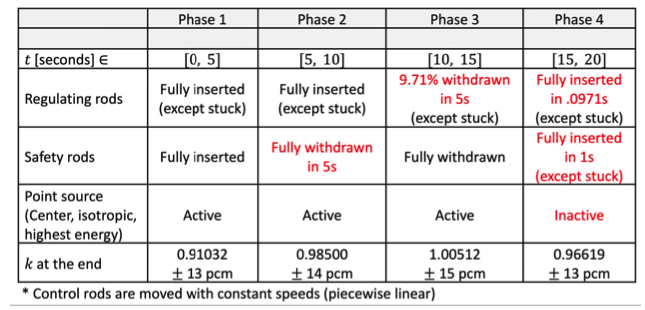
\includegraphics[width=\textwidth]{Figures/phases.png}
    \caption{The four phases of the CEMeNT challenge problem~\cite{psaap-presentation}; our work will focus on phase 1.}
    \label{fig:phases}
\end{figure}

\begin{figure}
    \centering
    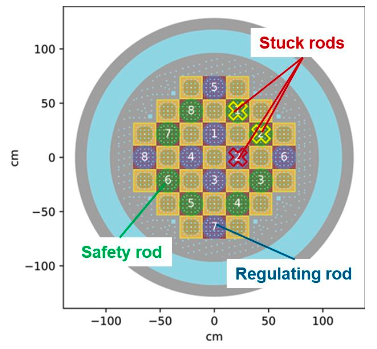
\includegraphics[scale=0.9]{Figures/smr.png}
    \caption{Cross-sectional view of the reactor test problem with rods highlighted~\cite{psaap-presentation}.}
    \label{fig:smr}
\end{figure}

\begin{figure}
    \centering
    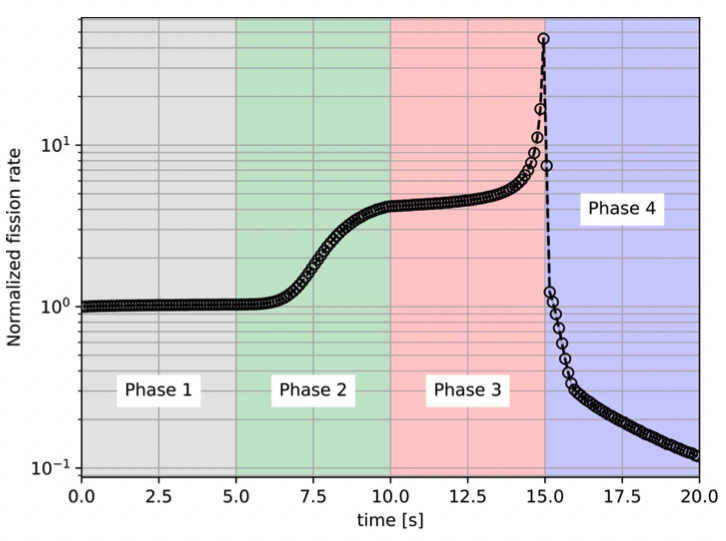
\includegraphics[width=\textwidth]{Figures/fission.png}
    \caption{Total fission rate results from MC/DC with $\sim 10^{10}$ particle histories~\cite{psaap-presentation}.}
    \label{fig:fission}
\end{figure}

By incorporating the framework into an existing and active codebase, we will be able to test the UQ and GSA performance when both the physics and tallying complexity of the simulations are scaled up. MC/DC's existing capabilities include 3D geometry; time-dependence; tallies such as flux, current, fission density, and Eddington factors; and variance reduction techniques such as weight windows are in active development by collaborators. We will be able to collaborate with the software's main developer, Ilham Variansyah, to incorporate methods developed in this PhD research into MC/DC such that a user could perform reliable UQ or GSA studies using a highly capable Monte Carlo radiation transport solver and evaluate computational scaling with increased physics and tally requirements. 